
%%%%%%%%%%%%%%%%%%%%%%% file typeinst.tex %%%%%%%%%%%%%%%%%%%%%%%%%
%
% This is the LaTeX source for the instructions to authors using
% the LaTeX document class 'llncs.cls' for contributions to
% the Lecture Notes in Computer Sciences series.
% http://www.springer.com/lncs       Springer Heidelberg 2006/05/04
%
% It may be used as a template for your own input - copy it
% to a new file with a new name and use it as the basis
% for your article.
%
% NB: the document class 'llncs' has its own and detailed documentation, see
% ftp://ftp.springer.de/data/pubftp/pub/tex/latex/llncs/latex2e/llncsdoc.pdf
%
%%%%%%%%%%%%%%%%%%%%%%%%%%%%%%%%%%%%%%%%%%%%%%%%%%%%%%%%%%%%%%%%%%%


\documentclass[runningheads,a4paper]{llncs}

\usepackage{amssymb}
\setcounter{tocdepth}{3}
\usepackage{graphicx}
\usepackage{xcolor}
\usepackage{hyperref}

\newcommand{\keywords}[1]{\par\addvspace\baselineskip
\noindent\keywordname\enspace\ignorespaces#1}

\begin{document}

\mainmatter  % start of an individual contribution

% first the title is needed
\title{TELEMETA, Web project for handling academic research sound archives}

% a short form should be given in case it is too long for the running head
\titlerunning{TELEMETA}

% the name(s) of the author(s) follow(s) next
%
% NB: Chinese authors should write their first names(s) in front of
% their surnames. This ensures that the names appear correctly in
% the running heads and the author index.
%
\author{Thomas Fillon\inst{1}
%
\thanks{This work was partially done inside the DIADEMS project funded by the national french agency ANR }%
\and Guillaume Pelerin\inst{1}
 \and Jos{\'e}phine Simonnot\inst{2}
}
%
%\authorrunning{Lecture Notes in Computer Science: Authors' Instructions}
% (feature abused for this document to repeat the title also on left hand pages)

% the affiliations are given next; don't give your e-mail address
% unless you accept that it will be published
\institute{PARISSON, \url{http://www.parisson.com}\\
\url{{thomas.fillon,guillaume.pellerin}@parisson.com}
\and 
CREM, LESC, CNRS UMR 7186, M.A.E. - Universit{\'e} Paris Ouest\\
\url{josephine.simonnot@??}}

%
% NB: a more complex sample for affiliations and the mapping to the
% corresponding authors can be found in the file "llncs.dem"
% (search for the string "\mainmatter" where a contribution starts).
% "llncs.dem" accompanies the document class "llncs.cls".
%

%\toctitle{Lecture Notes in Computer Science}
%\tocauthor{Authors' Instructions}
\maketitle


\begin{abstract}
The abstract should summarize the contents of the paper and should
contain at least 70 and at most 150 words. It should be written using the
\emph{abstract} environment.
\keywords{Sound archives, Ethnomusicology, Database, web platform, Metadata}
\end{abstract}


\section{Introduction}

In social sciences like anthropology or linguistic, researchers have to work on multiple type of multimedia documents like photos, videos, sound recordings or databases. The need to easily access, visualize and annotate such materials can be problematic given their diverse formats, sources and given their chronological nature.

Accessing audio archives materials with numerous collection of items of arbitrary duration ranging from a minute to several hours was a common issue shared by some laboratories from the french National Center on Scientific Research (CNRS) and involved in research on Ethnomusicoly. Those laboratories, the Research Center on Ethnomusicology (CREM),the Musical Acoustics Laboratory (LAM, UMR 7190) and the sound archives of the Mediterranean House of Human Sciences (MMHS) have decided to join together to develop a solution for managing, preserving, accessing and broadcasting their sound archives.

Beside the audio data, an efficient and dynamic management of the associated metadata is also required. Consulting metadata provide both an exhaustive access to valuable information about the source of the data and to the related work of peer researchers. Dynamically handling metadata enable to further and continuously improve the materials or to add new information in a collaborative manner. 

In light of those considerations, as no existing \emph{open-source} application was available, the need to specify and develop one has emerged. Since 2007, the CREM laboratory has been developing \emph{Telemeta}, a innovative, collaborative and interdisciplinary framework that both fits the professional requirements from sound archivists and human sciences researchers.

With the help and expertise of Parisson, a company specialized in the management of audio database, a first prototype of this web-based multimedia platform, named \emph{Telemeta} has been online since 2008 and enable to access sound archives of the CREM laboratory and their associated documentations \cite{telemetaCREM}.%\footnote{Archives sonores du CNRS, Musée de l'Homme, \url{http://archives.crem-cnrs.fr}}
 
\section{Telemeta architecture}

  
The main goal of \emph{Telemeta} is to facilitate the work of both researchers and archivists and to provide a convenient way to broadcast or distribute the digital audio collections.

\emph{Telemeta} architecture is flexible and can easily be adapted to particular database organization of a given sound archives. The compatibility with other systems is facilitated by the integration of the metadata standards protocols \emph{Dublin Core} and \emph{OAI-PMH} \cite{DublinCore,OAI-PMH}.

\emph{Telemeta} features multi-criteria text-based search engine and functions to easily navigate inside an audio item.
+ audio analysis (via TimeSide)
+ time markers for annotation and segmentation of instant or temporal region of the audio data.

Online sharing of the data enable a collaborative work of different partners with complementary skills and thus optimize the continuous process of knowledge gathering and enhancement of the database.

\subsection{Web interface to Audio database}
Django
Database model
Audio player with annotation capabilities see section~\ref{sec:metadata}
\subsection{Metadata}\label{sec:metadata}

One of the major challenge is the standardization of audio and metadata formats with the aim of long-term preservation and usage of the different materials. 

\begin{itemize}
\item Geographic and cultural informations (Location details, population/social group, ethnographic context)
\item Musical informations (style, composition, interprets, ...)
\item Archiving data (code and reference to the item)
\item Technical data (media type and duration)
\item Related media (any other material (images, video or text document associated with the audio item)
\end{itemize}


\begin{figure}[htbp]
  \centering
  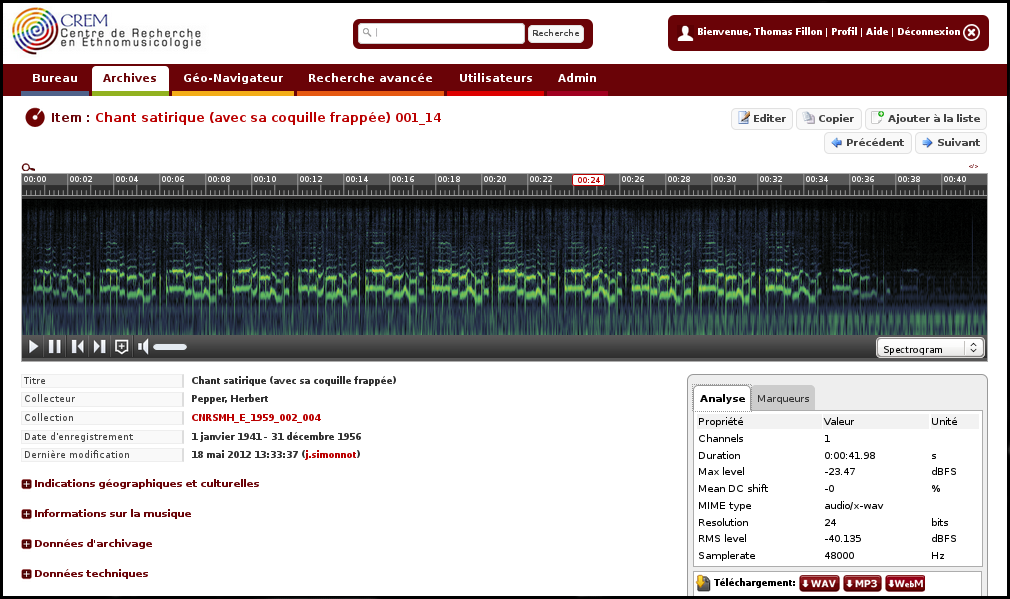
\includegraphics[width=12cm]{img/telemeta.png}
  \caption{Telemeta}
\end{figure}
\section{TimeSide}

\begin{figure}[htbp]
  \centering
  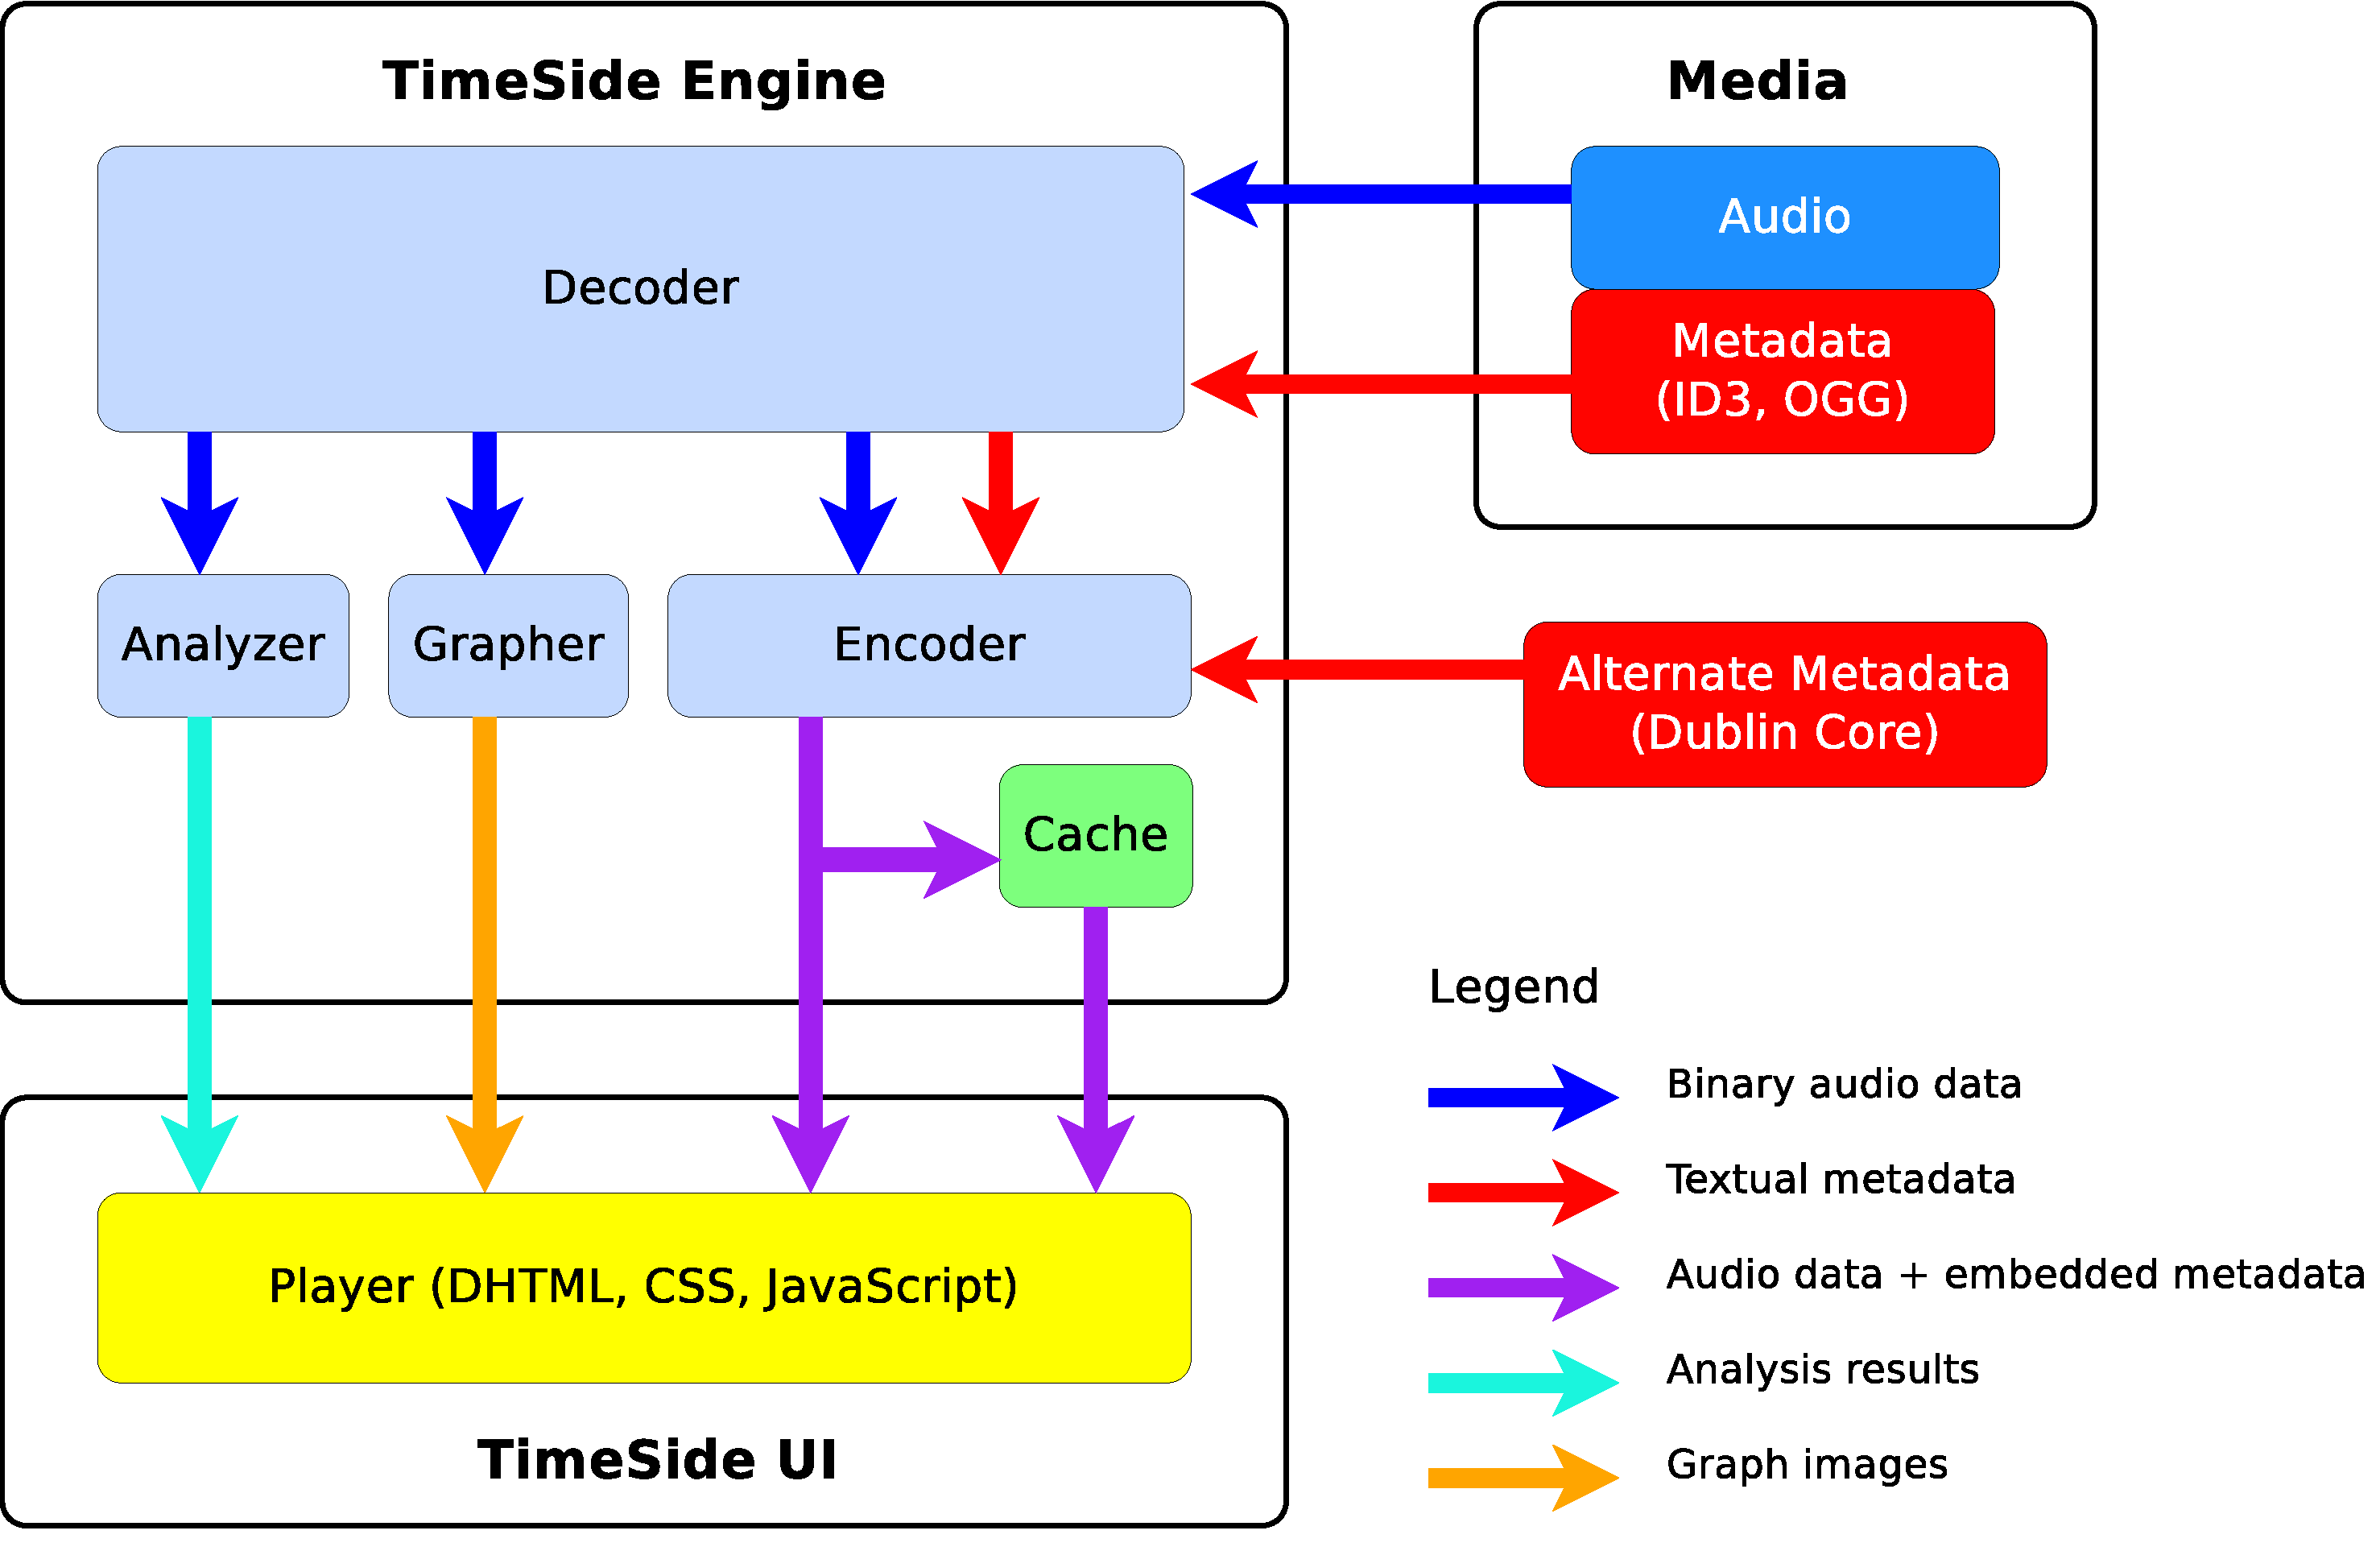
\includegraphics[width=12cm]{img/timeside_schema.pdf}
  \caption{TimeSide architecture}
\end{figure}
\subsection{Audio management}
Gstreamer, web player
with enhance visualization (waveform, spectrogram)
\subsection{Audio features extraction}
Include reference audio feature tools : Aubio + Yaafe + Vamp

flexible architecture 

\section{Current development and perspectives}
interdisciplinarity is further enhance by the Music Information Retrieval, Speech technology 
Diadems project
\subsection{Audio analysis}
Development of tools  to offer new audio analysis tool to ethnomusicologis research studies 
+ music similarity

\subsection{Automatic segmentation and classification}
\begin{itemize}
\item singing / talking voice segment
\item ...
\end{itemize}


\subsubsection*{Acknowledgments.} 
The authors would like to thanks all the people that have been involved in \emph{Telemeta} specification and development or have provide appreciated thoughts during discussions.



\bibliographystyle{splncs03}
\bibliography{cmmr_2013}


\end{document}
